%%% BEGIN CHAPTER 2 MD Simulations and MSM %%%

%% Paper title page %%
\chapter{Molecular dynamics simulations and Markov state modeling of potassium channel monomers}

\section{Introduction}
In a previous 650 ns simulation, the wild-type (WT) Kv1.2 pore domain monomer in POPC lipid bilayer was stable in a native-like state with a C$\alpha$-RMSD below 3\AA. \cite{gajewski2011} However, this simulation was relatively short compared with the timescale of membrane protein dynamics, which could extend from the micro to the millisecond timescale. \cite{booth1995} To further explore the conformational flexibility of the monomer, we carried out 16.2 $\mu$s of simulations at T=353 K using the specialized Anton computer designed for MD. \cite{shaw2009} The relatively high temperature was chosen to accelerate sampling while still reproducing the thermodynamics of membrane protein folding. \cite{ulmschneider2014}

\section{Methods}

\subsection{Preparation of Kv1.2 and KcsA monomer simulations}
For all systems, the initial structures for the monomers were taken from the tetrameric Kv1.2 X-ray crystal structure (PDB ID: 2A79) using only the pore domain of 99 amino acids corresponding to residues 323 –- 421 in 2A79 structure. \cite{long2005} The starting structure for KcsA monomer simulations was taken from the tetrameric KcsA X-ray crystal structure (PDB ID: 1R3J). \cite{zhou2003} All systems were prepared by using CHARMM-GUI’s Membrane Builder module (www.charmm-gui.org). \cite{jo2007, jo2008, jo2009, lee2016, wu2014} For Kv1.2, each system contained 70 palmitoyl-oleoyl-phosphatidylcholine (POPC) molecules per leaflet totaling up to 140 POPC molecules in total, and for KcsA, each system contained 70 1,2-dimyristoyl-sn-glycero-3-phosphatidylcholine (DMPC) molecules per leaflet totaling up to 140 DMPC molecules to match the NMR sample conditions. All systems were hydrated by creating a water box 17.5 \AA above and below the protein’s maximum and minimum Z-positions. In addition, the system was neutralized with 150 mM KCl. The system comprised a total of approximately 45,000 atoms.

For Kv1.2 simulations, a number of different simulations are aggregated and summarized in the table below.
\begin{table}[h]
\centering
	\caption{Simulation summary for Kv1.2}
	\begin{tabular}{cccc}
	\hline
    Simulation & Temperature (K) & Number of Trajectories & Trajectory length \\
	\hline                                                                 
	\begin{tabular}[c]{@{}c@{}} Anton\\ simulation \end{tabular} & 353.15  & 1 & 16.2 $\mu$s\\
	GPU & 303.15  & 10 & $\sim$9.7 $\mu$s\\
	\begin{tabular}[c]{@{}c@{}} Adaptive\\ sampling \end{tabular} & 303.15  & 4685 & 0.06$\mu$s\\
	\hline
	\textbf{Total:} & \textbf{N/A} & \textbf{4803} & \textbf{394 $\mu$s}
	\end{tabular}
	\label{table:ch2_t1}
	\end{table}
	
For KcsA simulations, 5 independent simulations of KcsA WT monomer were carried out at T = 353 K to enhance sampling. All simulations were run with the parameters described in \textit{Amber16 simulations} section below, and each simulation was run up to 6 $\mu$s. In total 30 $\mu$s of KcsA WT simulations were accumulated.

\subsection{Anton simulations}
A long-time simulation run on Anton \cite{shaw2009} was prepared through energy minimization and equilibrating the initial simulation system using CHARMM36 force field with NAMD. \cite{phillips2005} Each system was energy minimized for 1,000 steps and was slowly equilibrated by reducing restraints on protein backbone, sidechain, and lipids gradually over 5 ns as recommended by CHARMM-GUI. After initial equilibrations with the restraints, the system was freed from all restraints and run for 100 ns before preparing the system for running simulations on Anton. The temperature was set to 353 K to increase sampling, which has been shown to capture thermodynamics more computationally efficiently. \cite{ulmschneider2014} All bonds involving hydrogen atoms were constrained by M-SHAKE. Cut-off values for van der Waals and short-range electrostatic interactions were optimized by Anton guesser script. For long-range electrostatic interaction calculations, k-space Gaussian split Ewald method with a 64 x 64 x 64 mesh was used, and the long-range electrostatics were calculated every 6 fs. The integration time step was 2 fs for all simulations, and the r-RESPA integration method was employed. \cite{tuckerman1992}

\subsection{Amber16 simulations}
For all systems that were simulated with Amber16 GPU, hydrogen mass repartitioning (HMR) scheme was applied, where all hydrogen masses were increased to 3, allowing simulation timestep to increase from 2 to 4 fs. The systems were prepared as described in System Preparation section using CHARMM-GUI, and \textit{parmed.py} program was used to modify the system to accommodate the HMR scheme. For temperature control, Langevin thermostat was used with friction coefficient of 0.3 and T=303 K, and coordinates were printed out every 50 ps. van der Waals force switching function was used with switch on at 10 Å and cutoff at 12 Å. Berensden barostat is used with semi-isotropic at pressure 1 atm. The Berensden coupling constant is set to 0.5 ps.

\subsection{Time-lagged independent component and Markov state model analysis}
For all molecular dynamics (MD) simulation analysis, MDTraj 1.9.0 and MSMbuilder 3.8.0 were used. \citep{harrigan2017, mcgibbon2015} In the first steps of constructing a Markov State Model (MSM), proper set of reaction coordinates, and discretized states within the chosen reaction coordinates are necessary. For these purposes, time-lagged independent component analysis (tICA) was used. For TICA, a set of relevant features must be inputted to generate a set of low-dimensional linear combination of the input features. For this featurization step, pairwise distances of all C-$\alpha$ atoms of all residues was used, which resulted in 4,831 features. Then through TICA, dimensionality reduction was performed. Based on implied timescale analysis, 3 TICs with the slowest relaxation timescale was found to adequately describe our system (\textbf{Fig. \ref{fig:ch2_f1}}). All simulations were transformed and projected onto the 3 TICs found.

\begin{figure}[!ht]
\begin{center}
	\includegraphics[width=\textwidth]{figures/chapter2/Fig2-1_implied_timescale.png}
\end{center}
	\caption{\textbf{TICA analysis of Kv1.2 simulations.} The implied relaxation timescale of each TIC is plotted versus the number of TICs. The first 3 TICs are chosen as reaction coordinates to represent the folding coordinates of the simulations.}
	\label{fig:ch2_f1}
\end{figure}

To discretize a set of relevant conformations within the TIC space, K-Center clustering algorithm was used. The cutoff value for number of states was determined using the elbow method, where the momentum (sum of squared distances of samples to their closest centers) was plotted against the number of states. The number of states where the decrease in inertia became marginally less than a certain threshold was found. For Kv1.2, k=150 states was found to be appropriate for clustering (\textbf{Fig. \ref{fig:ch2_f2}}).

\begin{figure}[!ht]
\begin{center}
	\includegraphics[width=\textwidth]{figures/chapter2/Fig2-2_momentum.png}
\end{center}
	\caption{\textbf{Change in momentum over number of states.} Momentum is calculated as the sum of distances between each data point and its nearest centroid. To determine the optimal number of states for K-Center clustering method, the number of states where the momentum value begins to plateau is chosen. For our studies, k=150 states deemed to be optimal.}
	\label{fig:ch2_f2}
\end{figure}

In order to construct a MSM, the optimal lag time was needed for constructing the count matrix. By the definition of Markovianity, as the lag time increases, the implied timescale of the Markov State Model should become invariant. Through our implied timescale analysis, lag time of 20 ns was found to be appropriate, and the Markov State Model was constructed using this value.
	
\subsection{Adaptive sampling scheme}
For adaptive sampling, initial MSM was constructed using the Anton trajectory. Adaptive sampling scheme described previously by Bowman et. al was used. \citep{bowman2010} Briefly, in each round of simulations, 50 states with the lowest MSM populations were chosen and those chosen centroid conformations were used as seeds for an additional 60 ns of AMBER16 simulations using the CHARMM36 force field with Hydrogen Mass Repartitioning (HMR) scheme. After each round of simulations, new sets of TICs were calculated and a new MSM was constructed. In total, we accumulated 394 $\mu$s of simulations which are then used to create the final MSM for WT Kv1.2 monomer. 

\section{Results and Discussion}
\subsection{Potassium channel monomers are dynamical}
In a previous 650 ns MD simulation, the wild-type (WT) Kv1.2 pore domain monomer in POPC lipid bilayer was stable in a native-like state with a C$\alpha$-RMSD below 3 \AA. \cite{gajewski2011} However, this simulation is relatively short compared with the micro to the millisecond timescale of membrane protein dynamics. \citep{booth1995} To further explore the monomer’s conformational flexibility, we carried out 16.2 $\mu$s of simulations at T=353 K using the specialized Anton computer designed for simulations.\citep{shaw2009} The relatively high temperature was chosen to accelerate sampling while still reproducing the thermodynamics of membrane protein folding.

\begin{figure}[!ht]
\begin{center}
	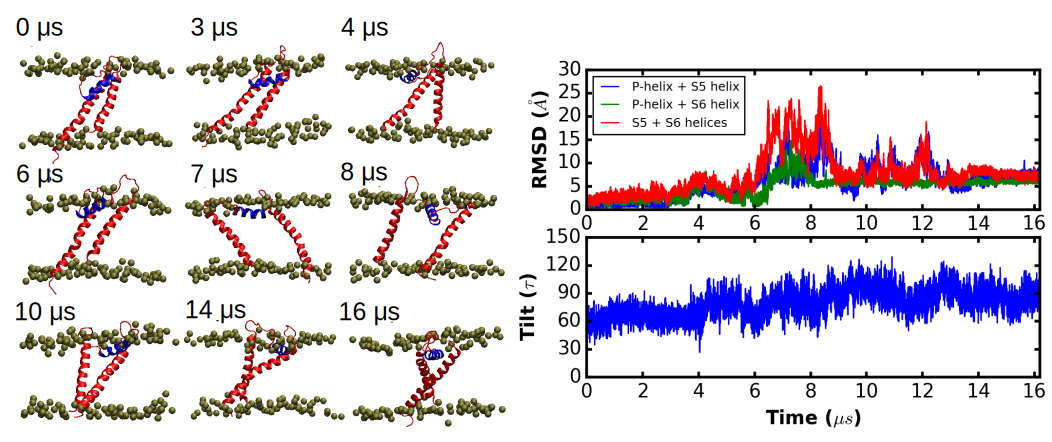
\includegraphics[width=\textwidth]{figures/chapter2/Fig2-3_anton.pdf}
\end{center}
	\caption{\textbf{Molecular dynamics simulation of Kv1.2 pore domain monomer in POPC lipid bilayer ran for 16.2 $\mu$s on Anton.} \textbf{Left}: Selected snapshots. \textbf{Right}: Pair-wise C$\alpha$-RMSD values for pairs of helices and the tilting angle of the pore helix.}
	\label{fig:ch2_f3}
\end{figure}

During the first 3 $\mu$s of the simulation, the structure was stable with a C$\alpha$-RMSD to the initial (native-like) state below 4 \AA (\textbf{Fig. \ref{fig:ch2_f3}}). Nevertheless, the p-helix became more parallel to the membrane during the first microsecond with the tilt angle increasing from 47$^{\circ}$ to 80$^{\circ}$ relative to the surface normal (\textbf{Fig. \ref{fig:ch2_f3}}). The average tilt angle over the entire 16.2 $\mu$s was 80$^{\circ}$ $\pm$ 10$^{\circ}$. At 4 $\mu$s, the 2 TM helices started to separate laterally with slightly different tilt angles due to their different lengths, leading to overall C$\alpha$-RMSD values greater than 4 \AA. 

Between 6 and 8 $\mu$s, all three helices separated (Fig. S1), but the p-helix remained helical and stayed nearly parallel to the membrane surface. This orientation allowed the polar and charged residues in the pore loop region to become more solvent exposed, while segregating the nonpolar residues. This result is qualitatively consistent with the previous thiol-labeling results, which indicated that the p-helix remains helical and resides at the water-lipid interface. \citep{delaney2014} Based on short simulations (650 ns) and thiol-labeling experimental data, the Kv1.3 monomer was inferred to retain native-like tertiary contacts. \citep{gajewski2011} In the long Anton simulation, however, the monomer is stable up to 3 $\mu$s with RMSD less than 4 \AA but also explores many other non-native states.

After 8 $\mu$s of simulations, residue D381 formed a salt bridge with a K398 that resides on top of the carboxy-terminal S6 helix. This salt bridge persisted for the last 8 $\mu$s and stabilized the interactions between the S6 and the p-helix. The amino terminal S5 helix eventually drifted towards the complex formed by the S6 with the p-helix, to produce an alternate structure. Interestingly, the salt bridge formed between the p-helix and S6 mimics a salt-bridge that is formed between p-helix of one monomer with the S6 helix of an adjacent monomer in the native tetramer (which does exist in the simulations). Salt bridges are known to be overly stabilized in simulations25 so the longevity of the D381-K398 bridge may be unrealistic. Nevertheless, the monomer spent a majority of time with the three helices in a non-native arrangement.

\subsection{Markov state modeling of Kv1.2 and KcsA monomer simulations}
To obtain a better estimate of the conformation ensemble of Kv1.2 monomers, an analysis based on Markov state models (MSM) was performed using 3 sets of simulations (\textbf{Table. \ref{table:ch2_t1}}): (1) 16.2 $\mu$s Anton simulation at T=353 K; (2) 10 independent 9 $\mu$s long simulations starting from the native state at T=303 K; (3) 100 rounds of adaptive sampling simulations (SI Methods) at T=303 K. A total of 394 $\mu$s of simulations was accumulated and used for time-structure Independent Component Analysis (TICA) and MSM analysis. \citep{molgedey1994, noe2015, noe2016, perezHernandez2013, schwantes2013}

Based on the MSM analysis, the population of native-like structures (C$\alpha$-RMSD < 4 Å) converged at 18\% (Fig. 2B, S2 bottom). This result further supports the finding that the native-like monomer conformation is present but is not predominant in lipid bilayer. While the two TM helices and the p-helix retained their helicity in all structures, the monomer prefers to be partially disordered. The p-helix remained parallel to the water-lipid interface, which is consistent with the thiol-labeling results. \citep{gajewski2011} Overall, the monomer existed as a heterogeneous ensemble of contacting and non-contacting helices.

To compare with the Kv1.2 simulations, and to enable a direct comparison with our experiments, simulations were conducted on KcsA pore domain monomers without the C-terminal tetramerization domain (PDB ID: 1R3J, residues 22 -- 124). The pore domain of KcsA and Kv1.2, comprising the pore loop and the 2 TMs, have 31\% sequence identity. This suggests that the gross dynamical features of the two proteins should be qualitatively similar. Five 5 $\mu$s trajectories were initiated from the native state at T=353 K. To compare with the Kv1.2 simulations, the KcsA trajectories were first projected onto the same set of TICs obtained from the Kv1.2 simulations and also aggregated with the Kv1.2 simulations to create a new set of common microstates. Although the sampling was less extensive as compared to Kv1.2, the general behavior of KcsA was similar. The KcsA monomer adopted a variety of native-like (44\%) and non-native structures, albeit with the three helices separated less than Kv1.2 helices (Figs. S5, S6). 

\section{Conclusion}

%% REVERT FIGURE NUMBERING %%
\renewcommand\thefigure{\thechapter.\arabic{figure}} 

%%% END CHAPTER 2 MD MSM %%%

